\documentclass[12pt,a4paper]{article}
\usepackage[UTF8]{ctex}
\usepackage{geometry}
\usepackage{hyperref}
\usepackage{graphicx}
\usepackage{booktabs}
\usepackage{pgfplots}
\pgfplotsset{compat=1.18}

\geometry{left=2.5cm,right=2.5cm,top=2.5cm,bottom=2.5cm}

\title{\textbf{医学影像多模态大语言模型\\安全性评估系统\\工作汇报}}
\author{谢跃进}
\date{\today}

\begin{document}

\maketitle

\tableofcontents
\newpage

\section{项目背景与目标}

\subsection{研究背景}

随着人工智能技术的快速发展，多模态大语言模型（MLLM）在医学影像分析领域展现出巨大潜力。本项目基于MIMIC-CXR大规模胸部X光数据集，研究视觉-语言模型在医学诊断报告自动生成任务中的表现和安全性。

项目使用LLaMA-Factory框架对Qwen3-VL系列模型进行微调，使其能够根据胸部X光图像自动生成医学诊断报告。为了评估模型的临床安全性和准确性，我们构建了一套自动化评估系统。

\subsection{项目目标}

本项目的主要目标包括：构建医学影像诊断报告自动生成系统，开发基于LLM的自动化评审机制，对模型生成的报告进行全面的质量评估，分析模型在临床应用中的安全性和可靠性。

\section{数据处理与模型训练}

\subsection{数据准备}

使用convert\_mimic\_to\_sharegpt.py脚本处理MIMIC-CXR原始数据。该脚本遍历所有患者的X光图像和对应的医学报告，将其转换为LLaMA-Factory所需的ShareGPT对话格式。处理流程包括：读取患者目录下的所有X光图像（JPG格式），匹配对应的医学报告文本文件，生成包含图像标记和诊断报告的对话数据。

最终生成19,972个训练样本和2,219个测试样本，训练集和测试集按9:1的比例划分，使用固定随机种子确保可重复性。每个样本包含1-2张胸部X光图像（正位片或正位+侧位）以及完整的放射科诊断报告，平均每个样本约1.5张图像。

\subsection{模型微调}

基于Qwen3-VL-8B-Instruct预训练模型进行全参数微调。训练策略采用冻结视觉编码器和多模态投影层的方式，仅微调语言模型部分，以保持视觉特征提取能力的同时专注于医学领域的文本生成。使用DeepSpeed ZeRO-3优化器支持大规模模型的分布式训练，有效降低显存占用并提高训练效率。

训练采用batch size为16（单卡8 × 梯度累积2），学习率1e-5，使用cosine学习率调度器并设置10\%的warmup步数。模型训练2个epoch，总计626个训练步，耗时约38分钟（2293秒）。训练过程中loss从初始的3.17逐步下降，最终收敛到0.992，表明模型在医学报告生成任务上取得了良好的拟合效果。训练吞吐量为17.4 samples/second。

\section{评估系统构建}

本阶段工作主要完成了三个核心系统的开发与部署，并在2,219个测试样本上进行了完整评估。

\subsection{模型评估系统}

构建了自动化的模型评估系统，使用微调后的Qwen3-VL-8B模型根据输入的胸部X光图像生成医学诊断报告。系统支持多张X光图像的Base64编码输入，默认并发数为20可处理大规模数据集，并实现了3次自动重试机制以应对API波动。评估过程中每20个样本自动保存中间结果确保数据安全。

\subsection{LLM评审系统}

开发了基于大语言模型的自动化评审机制，使用QwQ和Qwen3-235B-A22B两个模型作为专家评审员对生成的诊断报告进行详细评分和分析。评审维度包括临床准确性（是否识别出相同的病理特征）、否定词正确性（对"No pneumothorax"等否定表述的判断）、解剖位置准确性（病变定位是否正确）以及错误类型分析（遗漏、幻觉、定位错误、严重程度错误）。

系统支持100并发处理大幅提升评估效率，实现了5次智能重试机制和指数退避策略（重试间隔1、2、4、8、16秒），评审结果采用结构化JSON格式便于后续分析。系统会自动处理模型输出中的思维链标签（thinking tags），提取最终的评审结果。

\subsection{推理生成系统}

实现了诊断推理过程生成系统，该系统能够生成从X光图像到诊断结论的详细推理过程提供可解释性分析。系统支持双认证模式（Basic Auth和Direct API Key）并能自动根据部署环境选择合适的API端点和模型配置，并发处理能力可根据模型大小灵活调整（默认5-20并发）。

\section{实验结果与分析}

\subsection{整体性能}

在MIMIC-CXR测试集上完成了全面评估，基本情况如下：

\begin{table}[h]
\centering
\begin{tabular}{ll}
\toprule
\textbf{指标} & \textbf{数值} \\
\midrule
测试样本数 & 2,219 \\
评估成功率 & 100\% \\
并发处理能力 & 20-100 \\
Judge模型数量 & 2个（QwQ、Qwen3-235B-A22B） \\
\bottomrule
\end{tabular}
\caption{评估系统整体性能}
\end{table}

\subsection{两个Judge模型的评分对比}

为了全面评估模型性能，我们使用了两个不同的大语言模型作为评审专家，从不同角度评估报告质量。

\begin{table}[h]
\centering
\begin{tabular}{lcc}
\toprule
\textbf{指标} & \textbf{QwQ} & \textbf{Qwen3-235B-A22B} \\
\midrule
平均分（满分10分） & 4.62 & 3.70 \\
0-2分比例 & 0.6\% & 4.2\% \\
2-4分比例 & 50.9\% & 71.0\% \\
4-6分比例 & 9.7\% & 2.8\% \\
6-8分比例 & 23.2\% & 6.6\% \\
8-10分比例 & 15.5\% & 15.3\% \\
\bottomrule
\end{tabular}
\caption{两个Judge模型的评分统计}
\end{table}

对比发现，Qwen3-235B-A22B作为评审员明显更加严格，平均分低0.92分；两个模型对高质量报告（8-10分）的判断高度一致，均在15\%左右；在中等分数段（4-8分），两个模型的评分标准存在显著差异，反映了不同评审视角。

\subsection{分数分布可视化}

\begin{figure}[h]
\centering
\begin{tikzpicture}
\begin{axis}[
    ybar,
    bar width=10pt,
    xlabel={分数区间},
    ylabel={样本数量},
    symbolic x coords={0-2, 2-4, 4-6, 6-8, 8-10},
    xtick=data,
    legend pos=north west,
    ymin=0,
    ymax=1700,
    width=13cm,
    height=8cm,
    enlarge x limits=0.2,
    ylabel style={font=\small},
    xlabel style={font=\small},
    legend style={font=\small},
]
\addplot[fill=blue!60] coordinates {(0-2,14) (2-4,1130) (4-6,216) (6-8,515) (8-10,344)};
\addplot[fill=red!60] coordinates {(0-2,94) (2-4,1575) (4-6,63) (6-8,147) (8-10,340)};
\legend{QwQ（平均分4.62）, Qwen3-235B-A22B（平均分3.70）}
\end{axis}
\end{tikzpicture}
\caption{两个Judge模型的分数分布对比}
\end{figure}

从图中可以看出，Qwen3-235B-A22B评分更严格（平均分低0.92分），两个模型对优秀样本（8-10分）的判断一致性高（15\%左右），中等分数段（4-8分）差异明显，反映不同评审标准。

\subsection{结果分析}

通过对2,219个样本的评估结果分析，我们发现以下特点。

根据QwQ的评分，超过50\%的样本得分在2-4分区间，说明模型在临床细节准确性上还有较大提升空间。主要错误类型包括遗漏关键发现（模型容易忽略报告中提到的重要病理特征，如心脏肥大、肺不张等）、幻觉现象（在正常报告中错误地识别出不存在的病变）、严重程度判断错误（将"severe"误判为"mild"或相反，影响临床决策）以及解剖定位错误（混淆左右肺叶、上下叶位置）。

约15\%的样本达到8-10分的高分水平，这表明模型在部分案例上已经接近专家水平具备一定的临床应用潜力。两个Judge模型对高质量报告的判断高度一致，说明在明显优秀的案例上不同评审标准的差异较小。

\subsection{典型案例分析}

为了更直观地展示模型的表现，我们从不同分数区间各选取一个代表性案例进行详细分析。

\subsubsection{案例1：严重诊断错误（1.5分）}

\noindent\textbf{样本信息：}Sample ID 720

\noindent\textbf{输入图像：}

\begin{figure}[h]
\centering
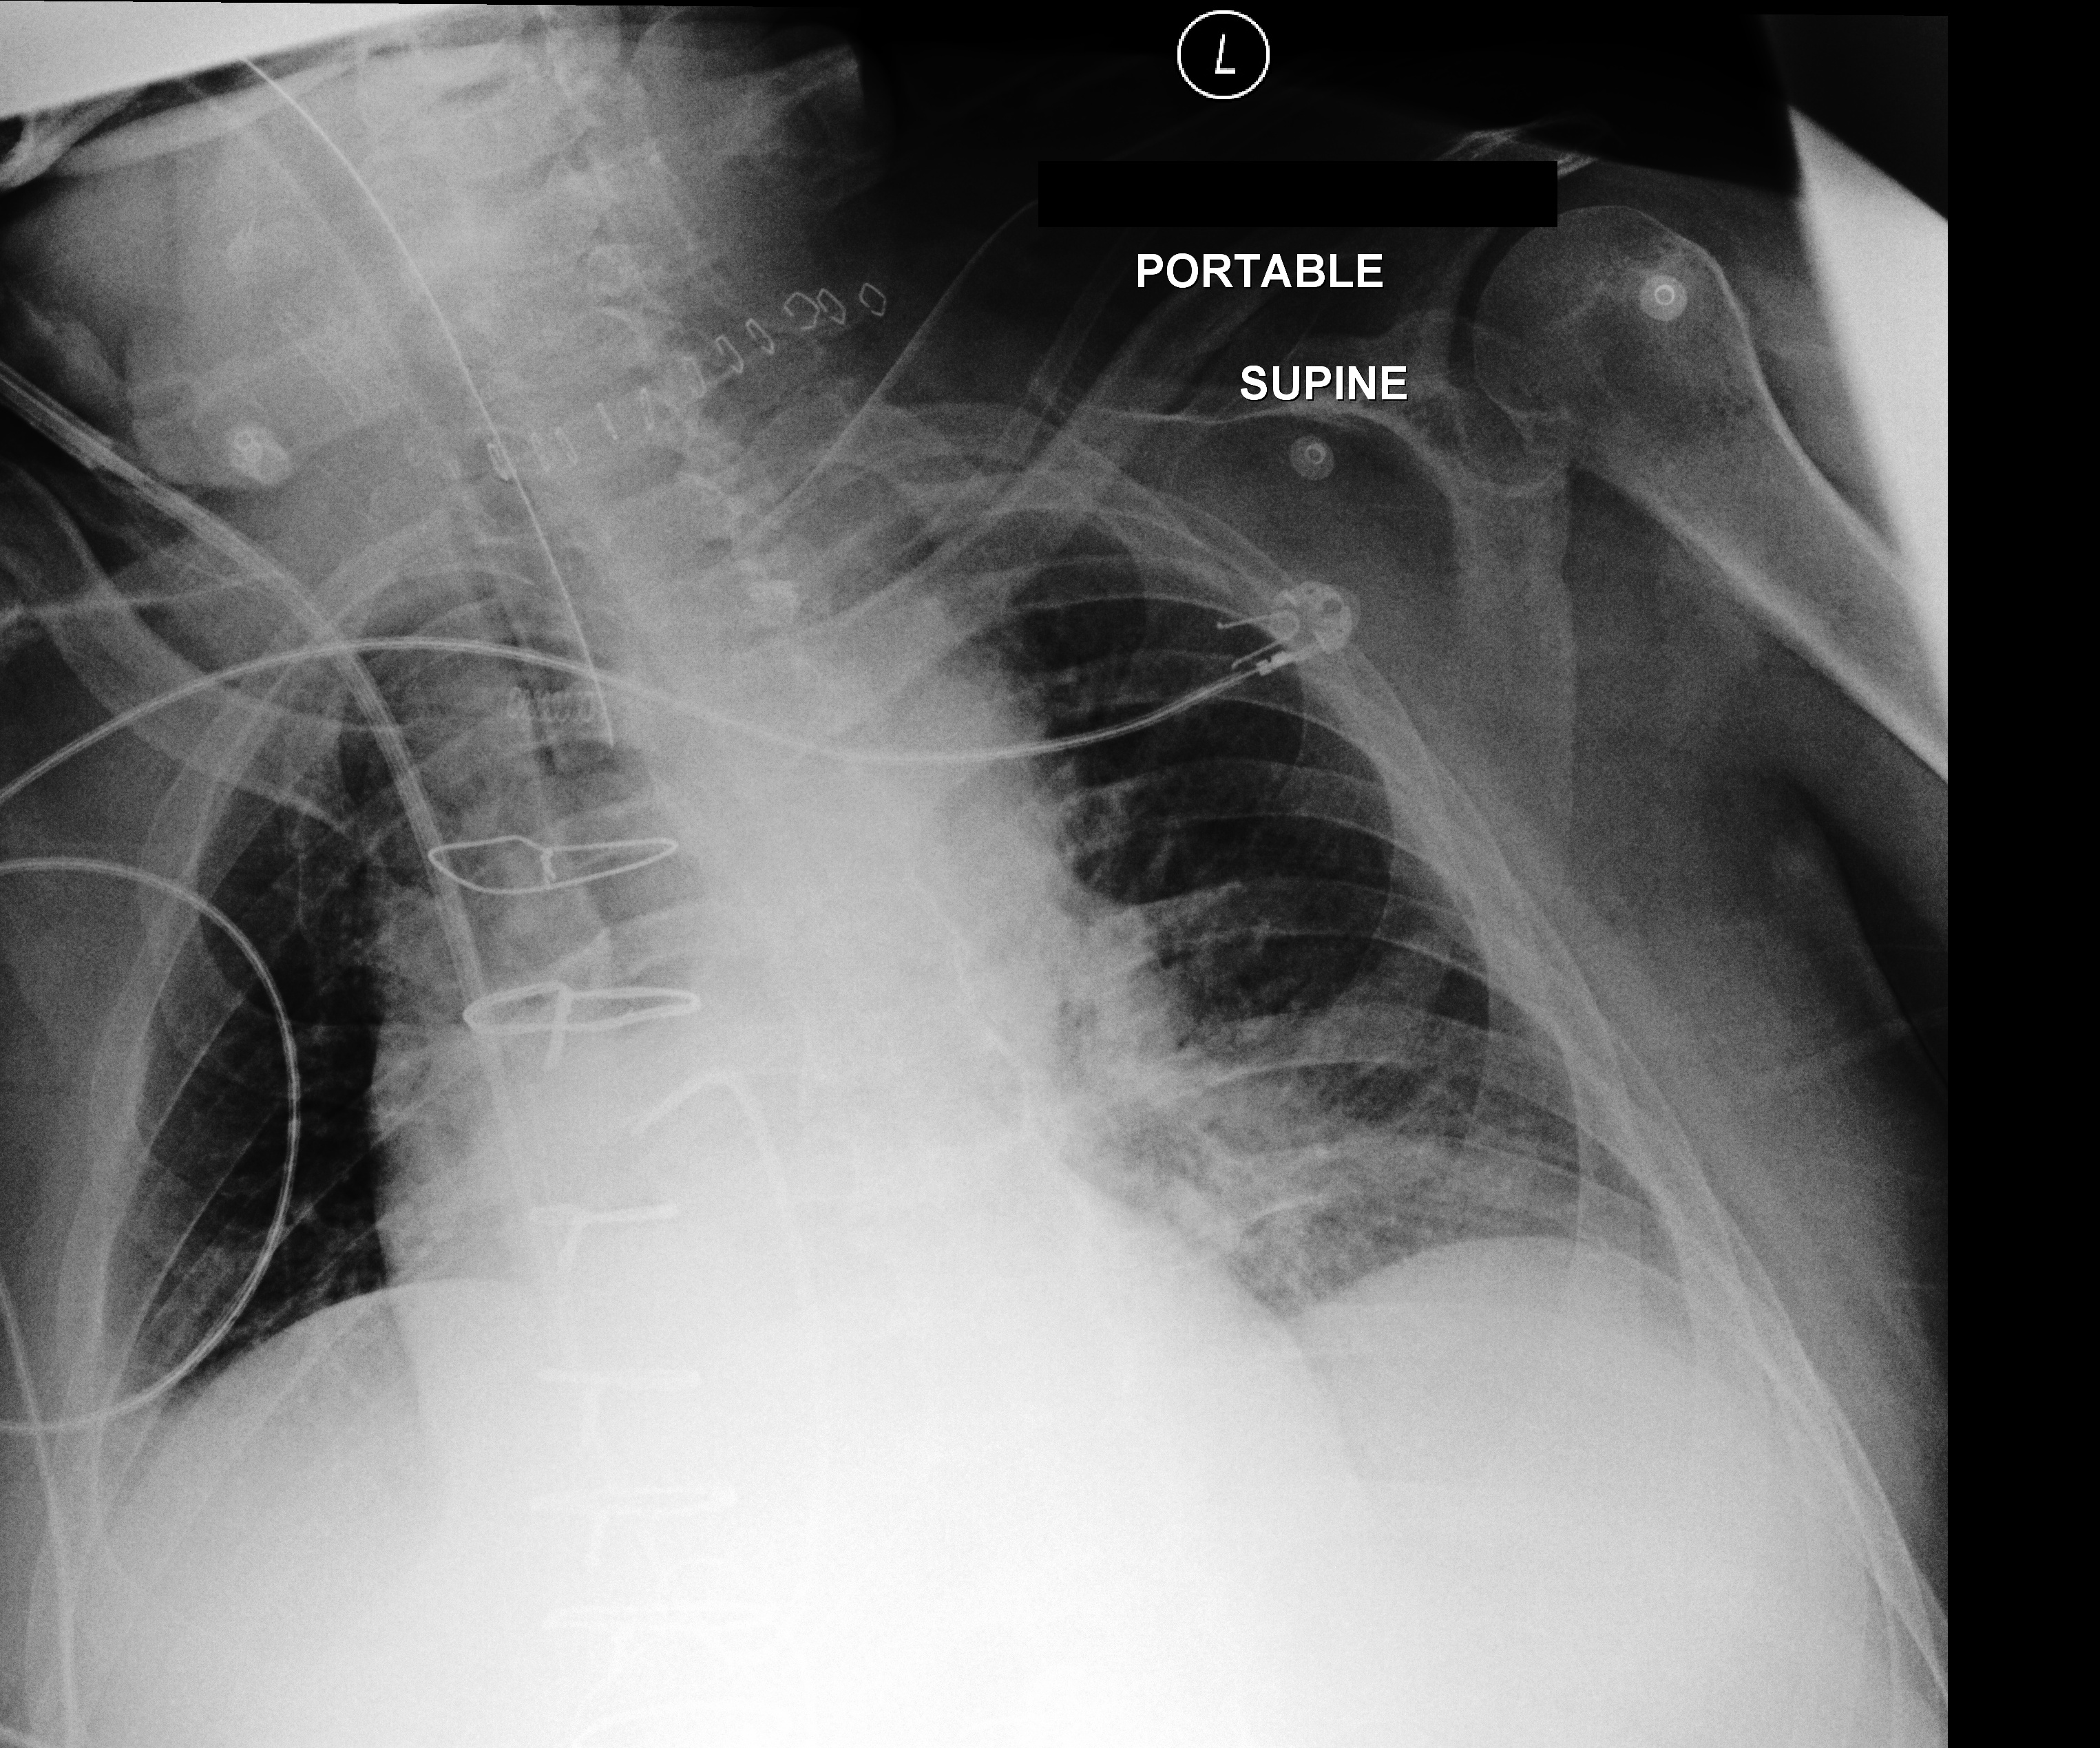
\includegraphics[width=0.6\textwidth]{images/sample_720_1.jpg}
\end{figure}

\noindent\textbf{诊断报告对比：}

\begin{table}[h]
\small
\begin{tabular}{p{0.47\textwidth}|p{0.47\textwidth}}
\toprule
\textbf{Ground Truth} & \textbf{模型预测} \\
\midrule
WET READ: Interval placement of an endotracheal tube, which terminates in the mid thoracic trachea, and pulmonary artery catheter, which terminates in the right pulmonary artery. Low lung volumes, with prominence of the cardiac silhouette... & FINAL REPORT: Compared to the prior study there is no significant interval change. IMPRESSION: No change. \\
\midrule
\multicolumn{2}{l}{\textbf{评分：}1.5/10.0 \quad \textbf{错误类型：}重大遗漏} \\
\bottomrule
\end{tabular}
\end{table}

\noindent\textbf{分析：}模型的预测极其简略，仅提到"无明显变化"。而Ground Truth详细描述了气管插管、肺动脉导管的位置，以及心脏轮廓增大等关键临床发现。模型完全遗漏了这些重要的医疗设备位置信息和病理特征，属于严重的诊断错误。

\subsubsection{案例2：主要错误（2.0分）}

\noindent\textbf{样本信息：}Sample ID 1124

\noindent\textbf{输入图像：}

\begin{figure}[h]
\centering
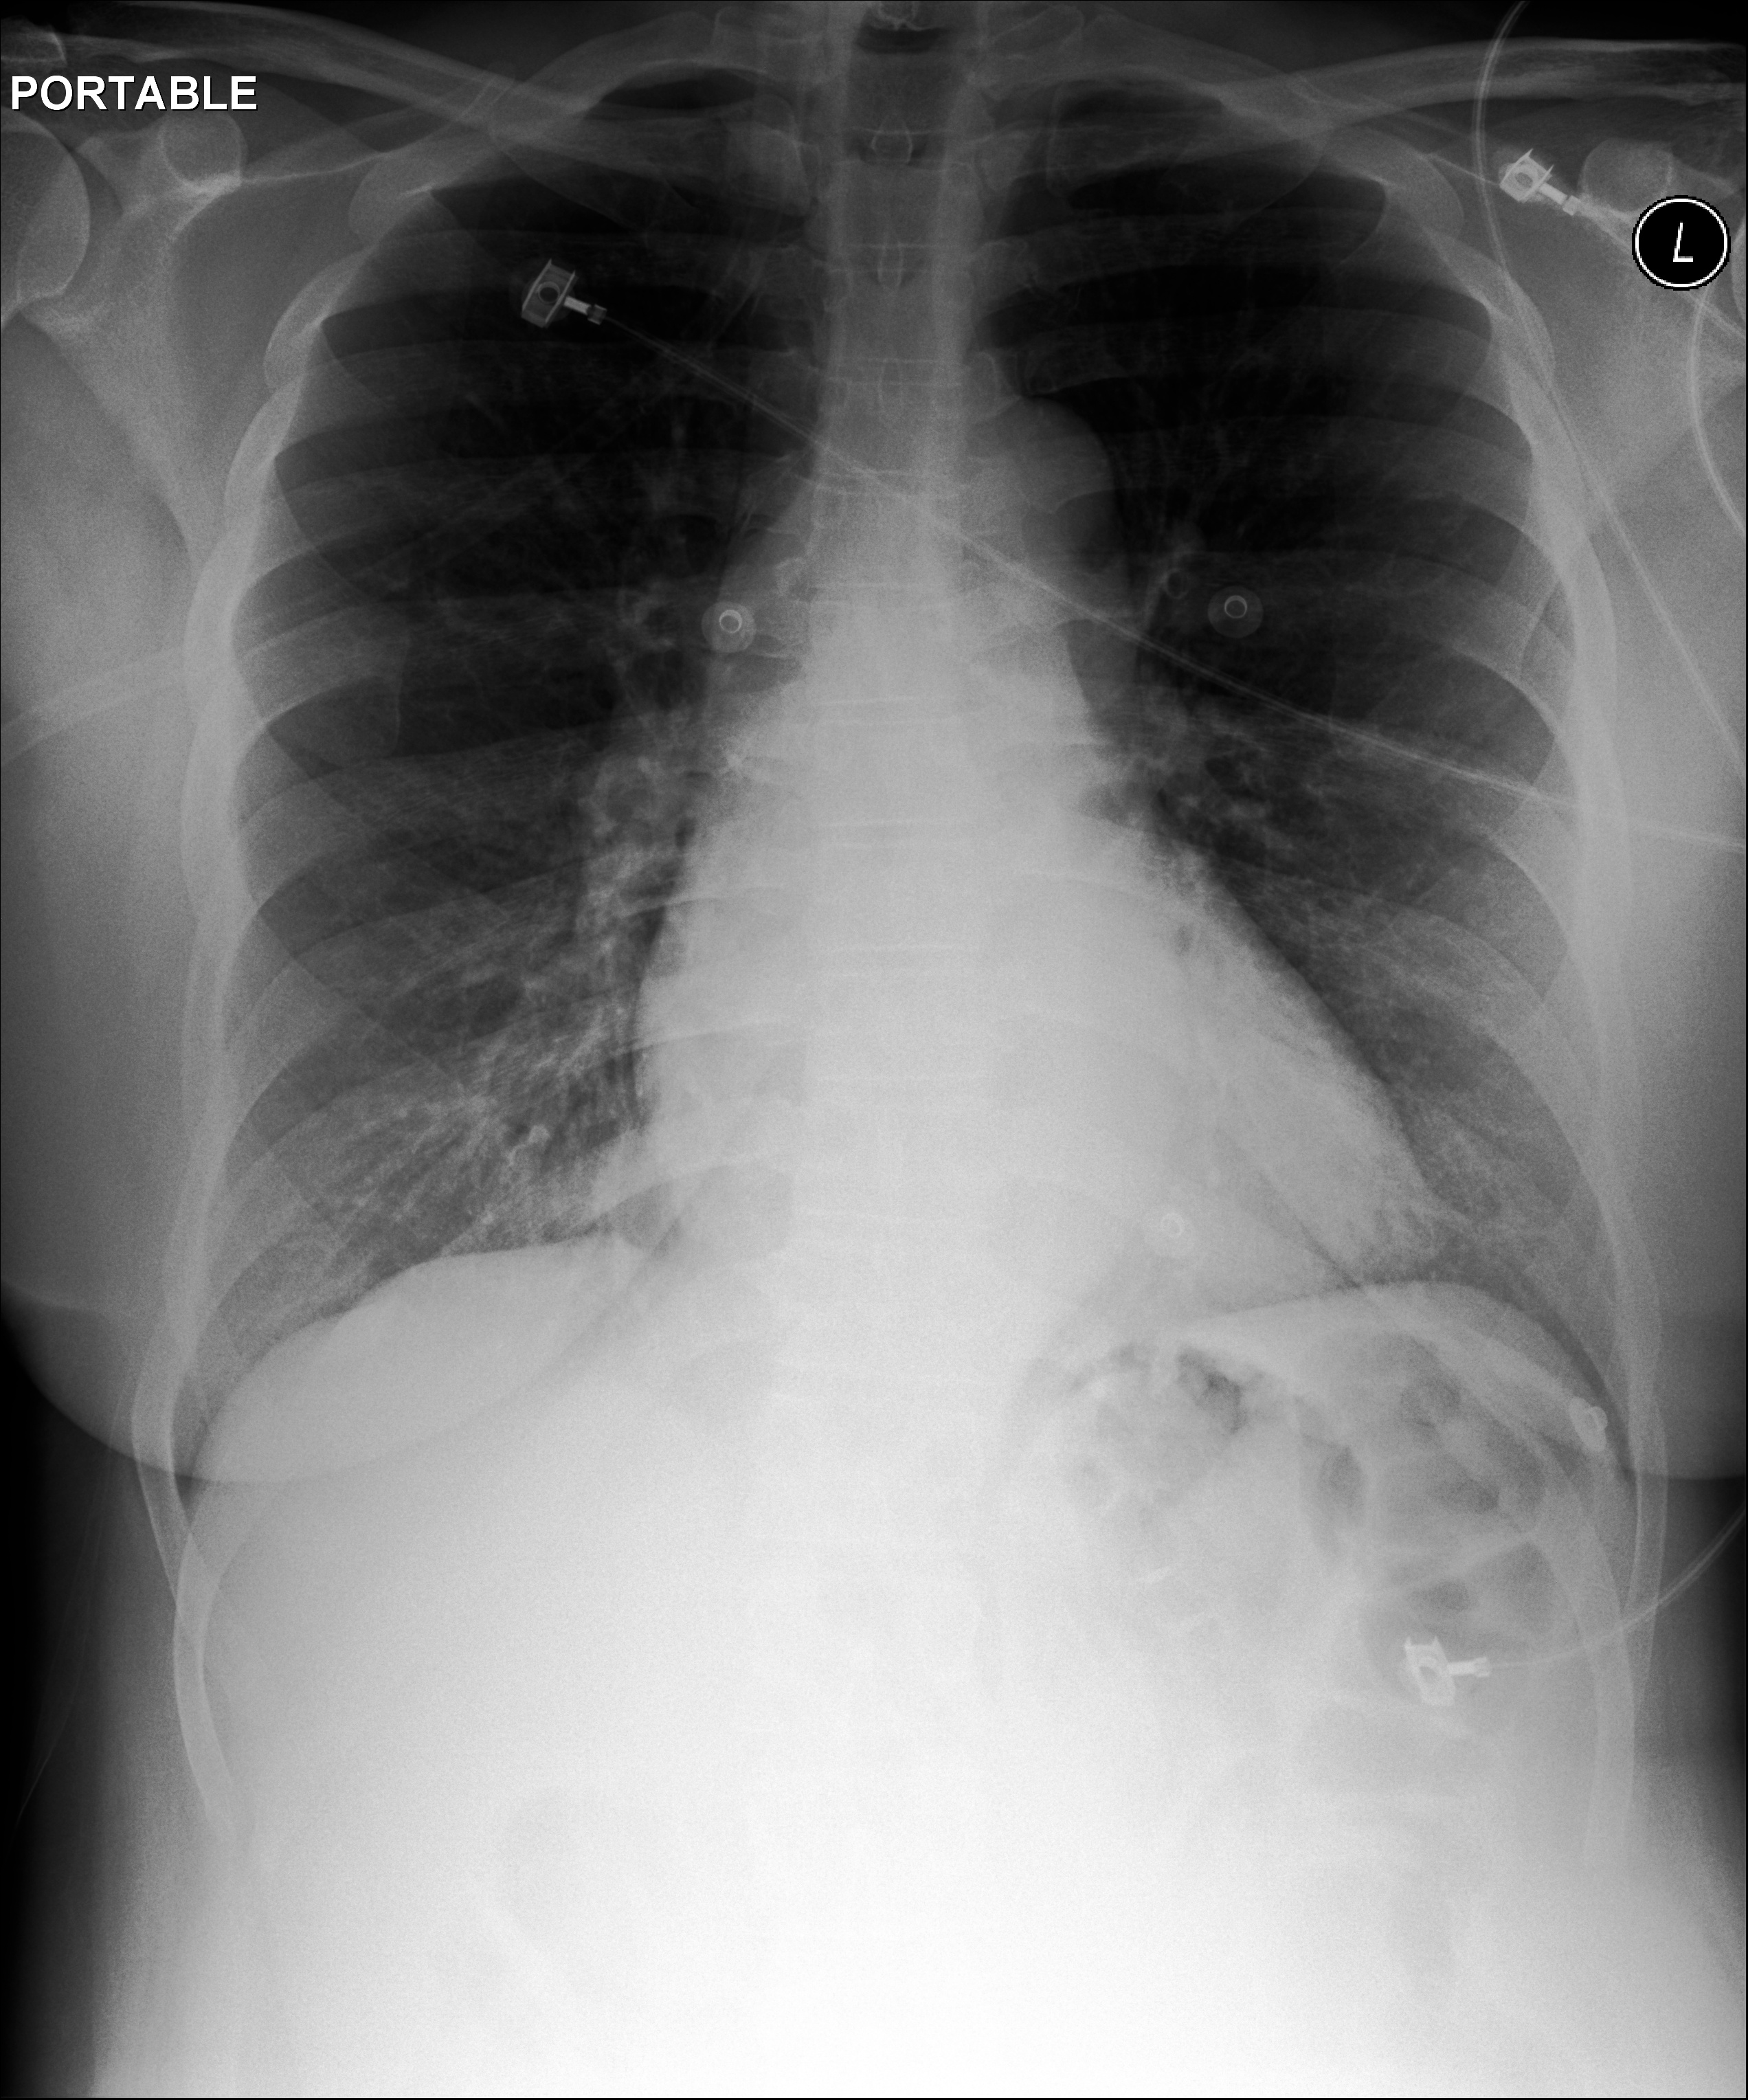
\includegraphics[width=0.6\textwidth]{images/sample_1124_1.jpg}
\end{figure}

\noindent\textbf{诊断报告对比：}

\begin{table}[h]
\small
\begin{tabular}{p{0.47\textwidth}|p{0.47\textwidth}}
\toprule
\textbf{Ground Truth} & \textbf{模型预测} \\
\midrule
FINDINGS: The lungs are clear. The cardiomediastinal silhouette is within normal limits for technique. No acute osseous abnormality is identified. IMPRESSION: No acute cardiopulmonary process. & IMPRESSION: Moderate cardiomegaly is stable. There is no pneumothorax or pleural effusion. Bibasilar atelectasis have improved. Aortic knob calcification is unchanged. \\
\midrule
\multicolumn{2}{l}{\textbf{评分：}2.0/10.0 \quad \textbf{错误类型：}幻觉} \\
\bottomrule
\end{tabular}
\end{table}

\noindent\textbf{分析：}Ground Truth明确指出肺部清晰、心脏轮廓正常、无急性病变。但模型却幻觉出三个不存在的发现：中度心脏肥大、双侧基底部肺不张、主动脉结钙化。这是典型的幻觉现象，模型在正常图像中错误地识别出病变，存在较大的临床风险。

\subsubsection{案例3：细节错误（5.0分）}

\noindent\textbf{样本信息：}Sample ID 1258

\noindent\textbf{输入图像：}

\begin{figure}[h]
\centering
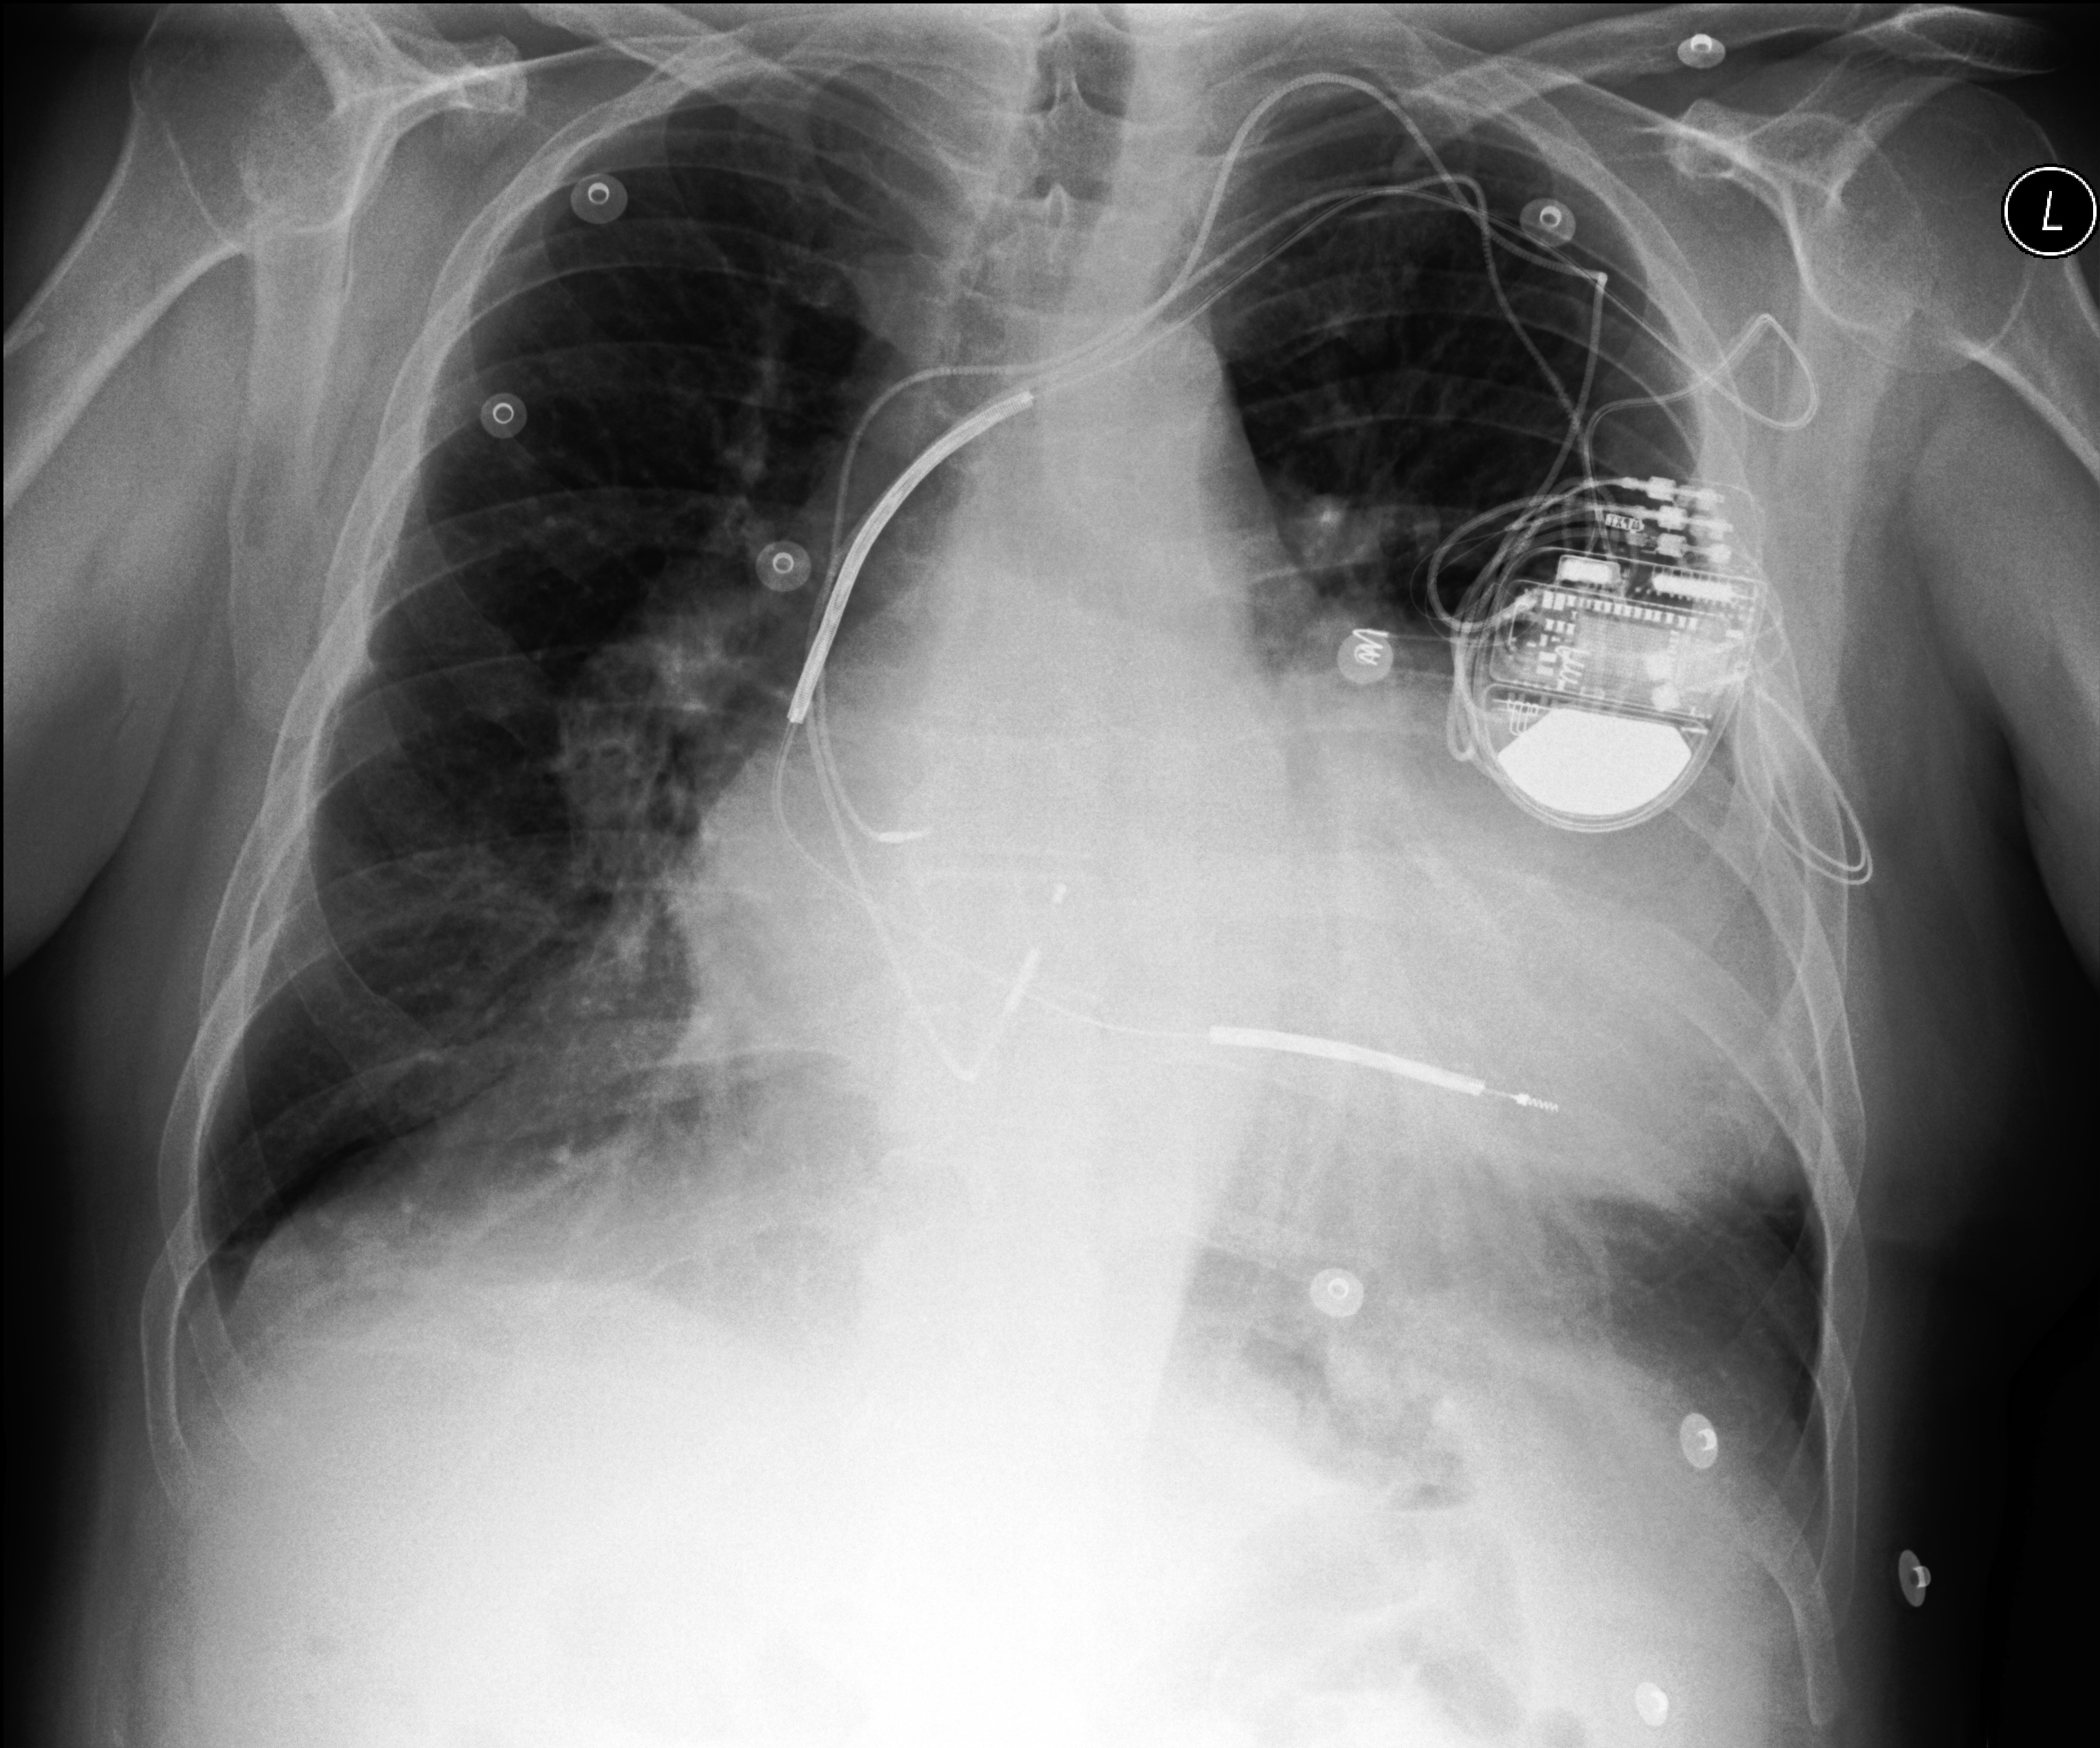
\includegraphics[width=0.45\textwidth]{images/sample_1258_1.jpg}
\hfill
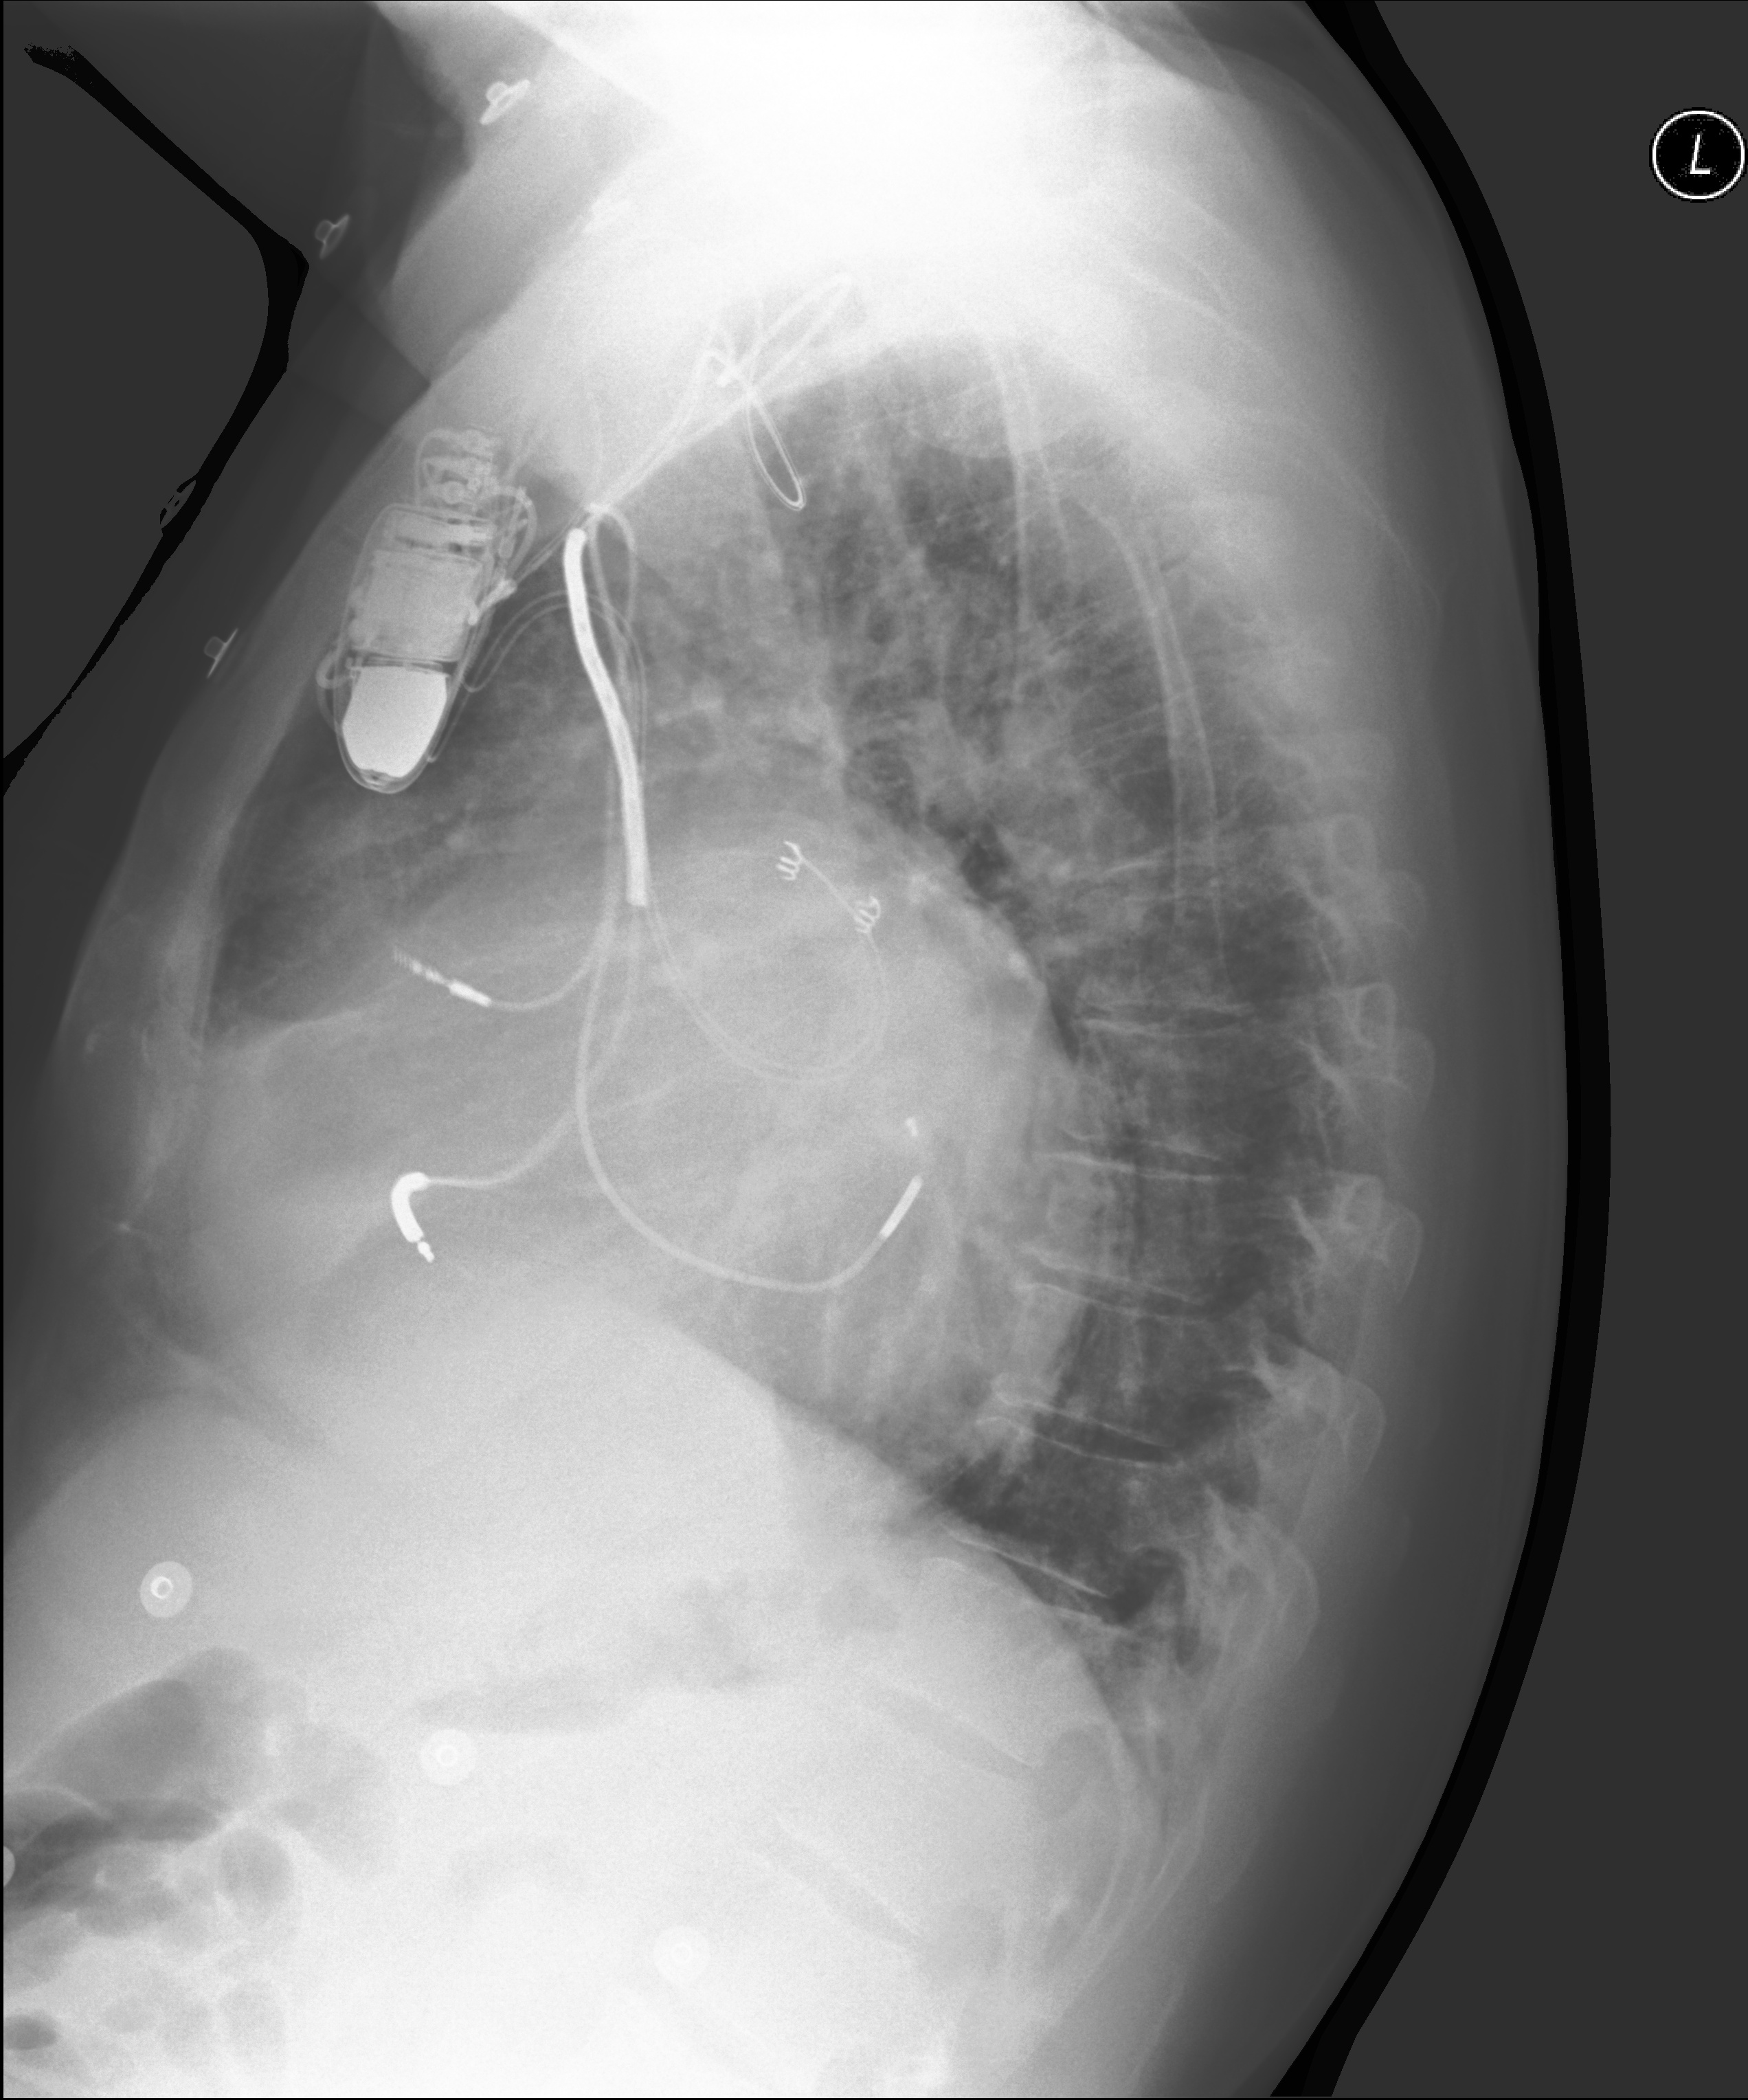
\includegraphics[width=0.45\textwidth]{images/sample_1258_2.jpg}
\end{figure}

\noindent\textbf{诊断报告对比：}

\begin{table}[h]
\small
\begin{tabular}{p{0.47\textwidth}|p{0.47\textwidth}}
\toprule
\textbf{Ground Truth} & \textbf{模型预测} \\
\midrule
Left-sided AICD device is noted with leads terminating in the regions of the right atrium, right ventricle and coronary sinus, unchanged. Severe cardiomegaly is again noted. Mediastinal and hilar contours are unchanged. No pulmonary edema... & Dual-lead left-sided pacemaker is unchanged in position. Lung volumes are low. There is mild cardiomegaly with a left ventricular predominance. The aorta is tortuous. There is no pleural effusion or pneumothorax... \\
\midrule
\multicolumn{2}{l}{\textbf{评分：}5.0/10.0 \quad \textbf{错误类型：}遗漏、幻觉、严重程度错误} \\
\bottomrule
\end{tabular}
\end{table}

\noindent\textbf{分析：}模型正确识别了起搏器和心脏肥大，但存在三个问题：遗漏了双侧肺底肺不张；幻觉出主动脉迂曲；将"严重心脏肥大"误判为"轻度心脏肥大"。严重程度的错误判断可能影响临床决策。

\subsubsection{案例4：轻微差异（6.0分）}

\noindent\textbf{样本信息：}Sample ID 1065

\noindent\textbf{输入图像：}

\begin{figure}[h]
\centering
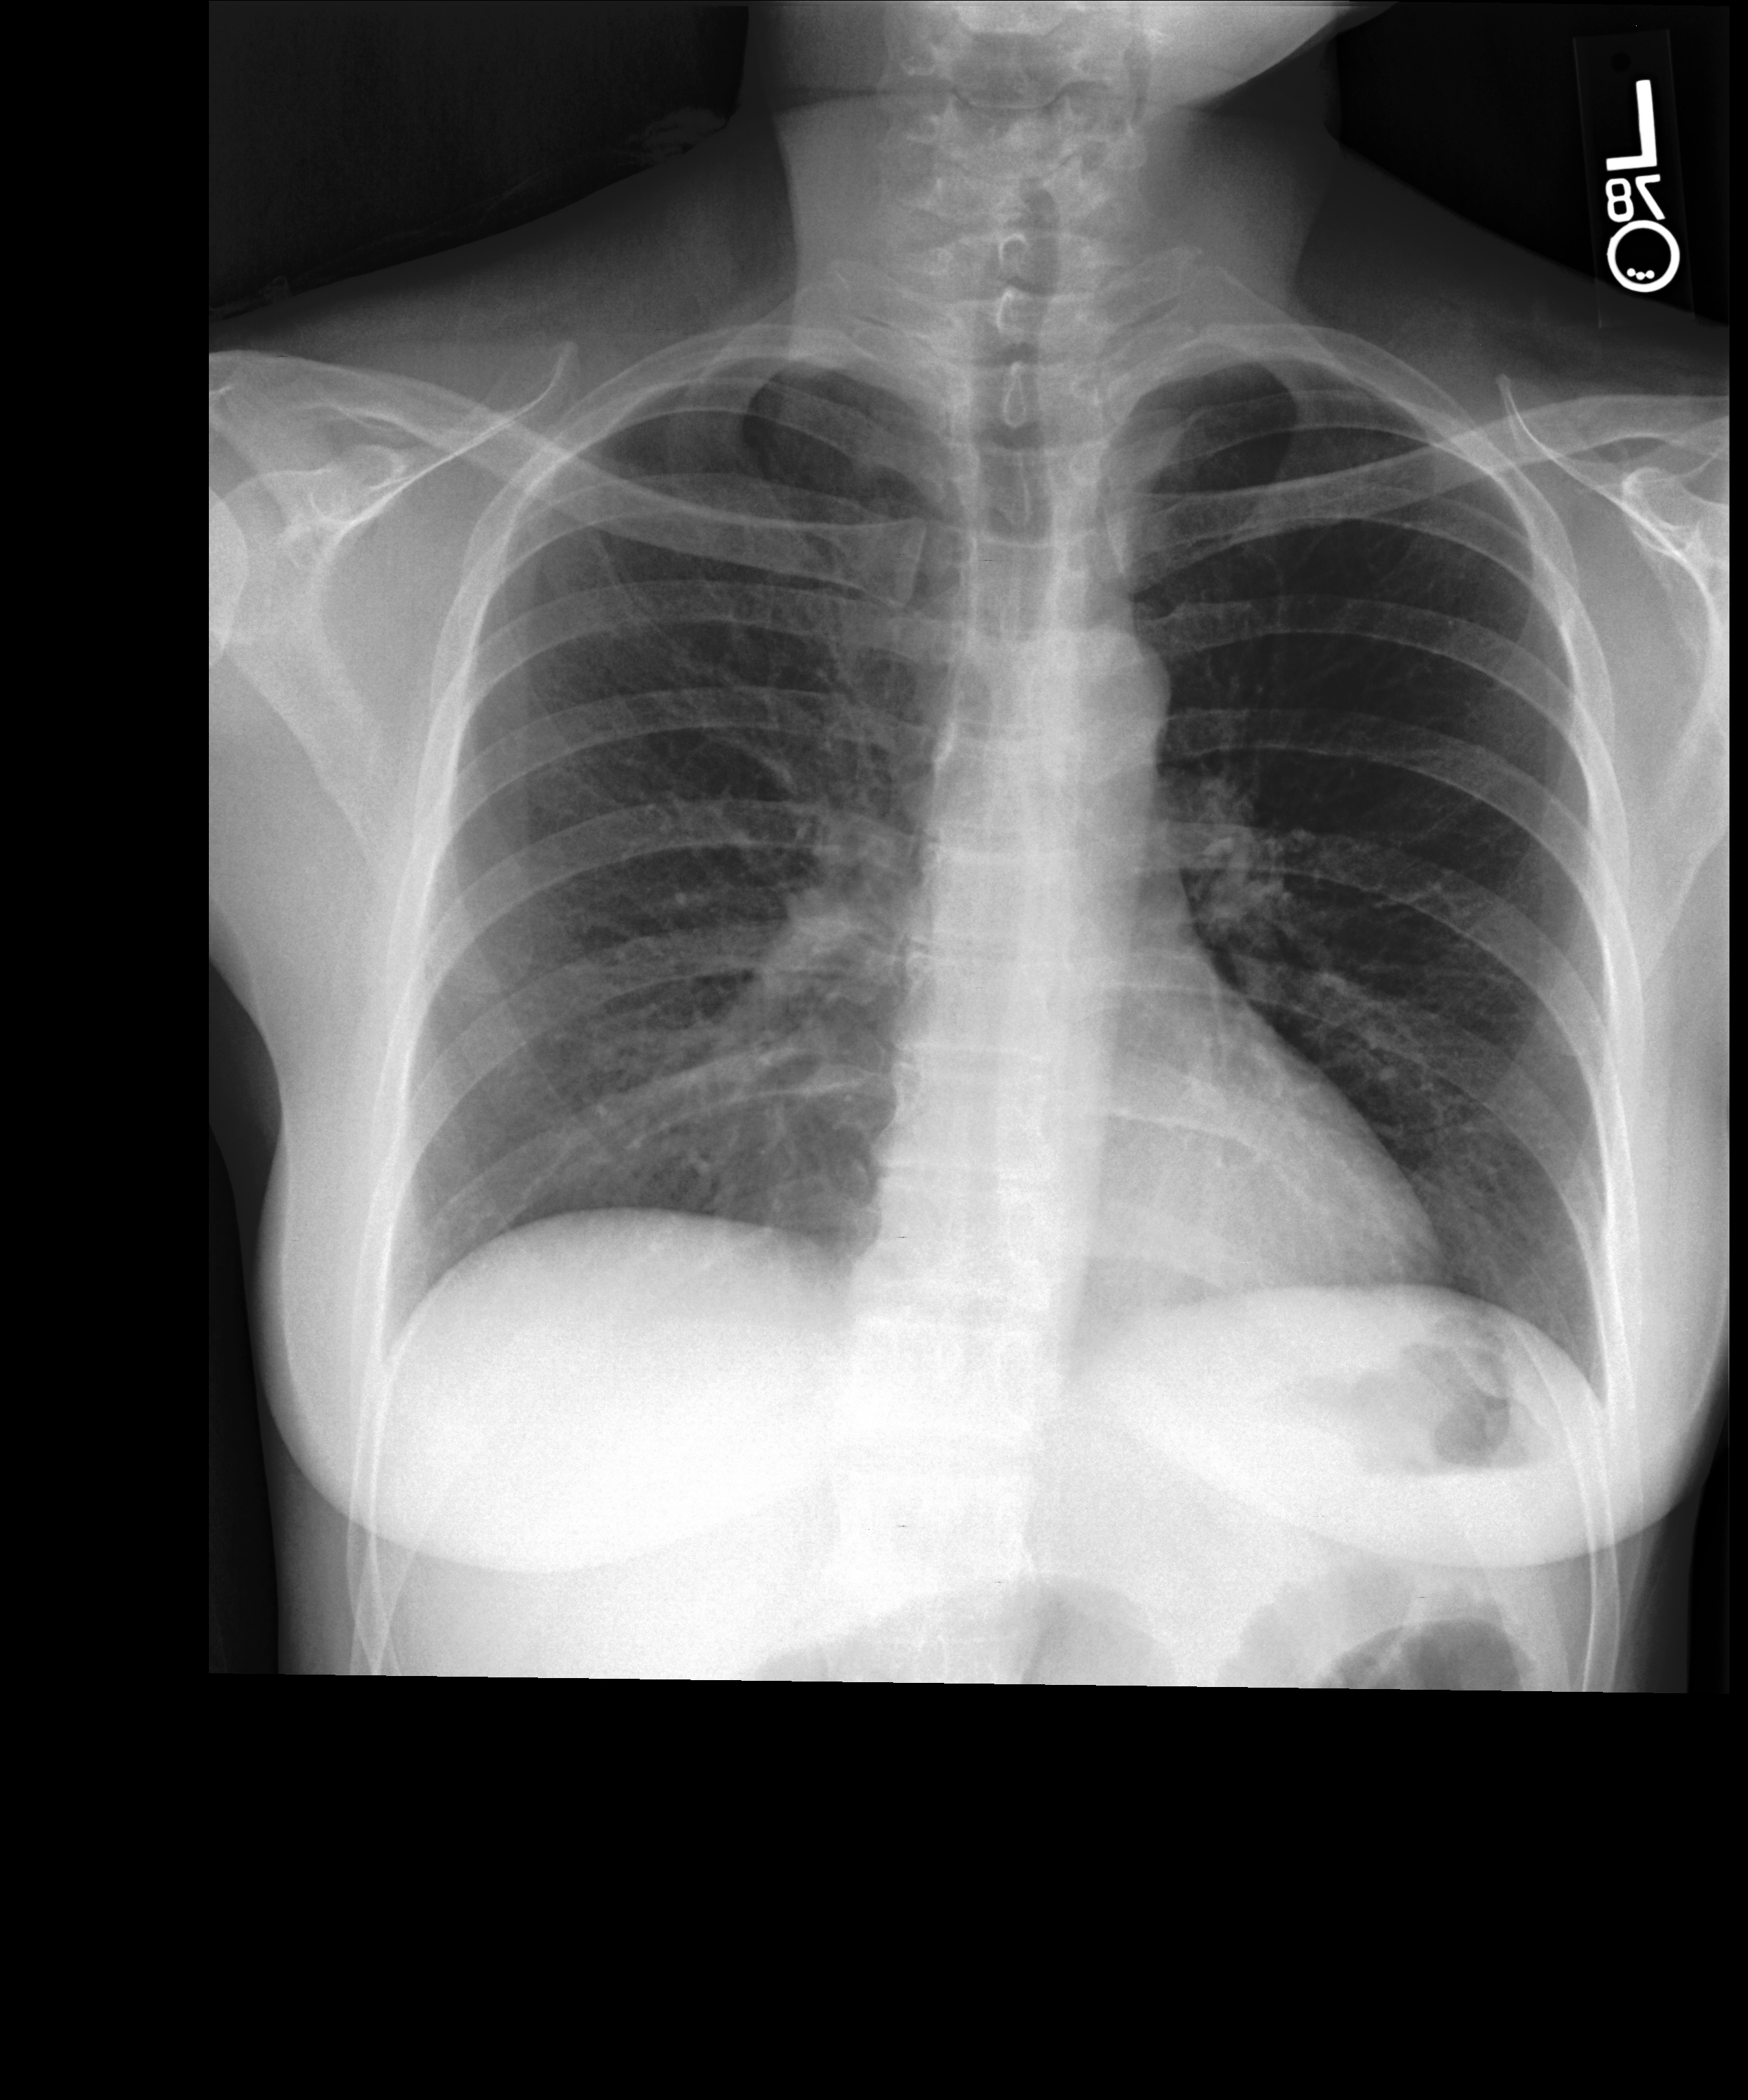
\includegraphics[width=0.45\textwidth]{images/sample_1065_1.jpg}
\hfill
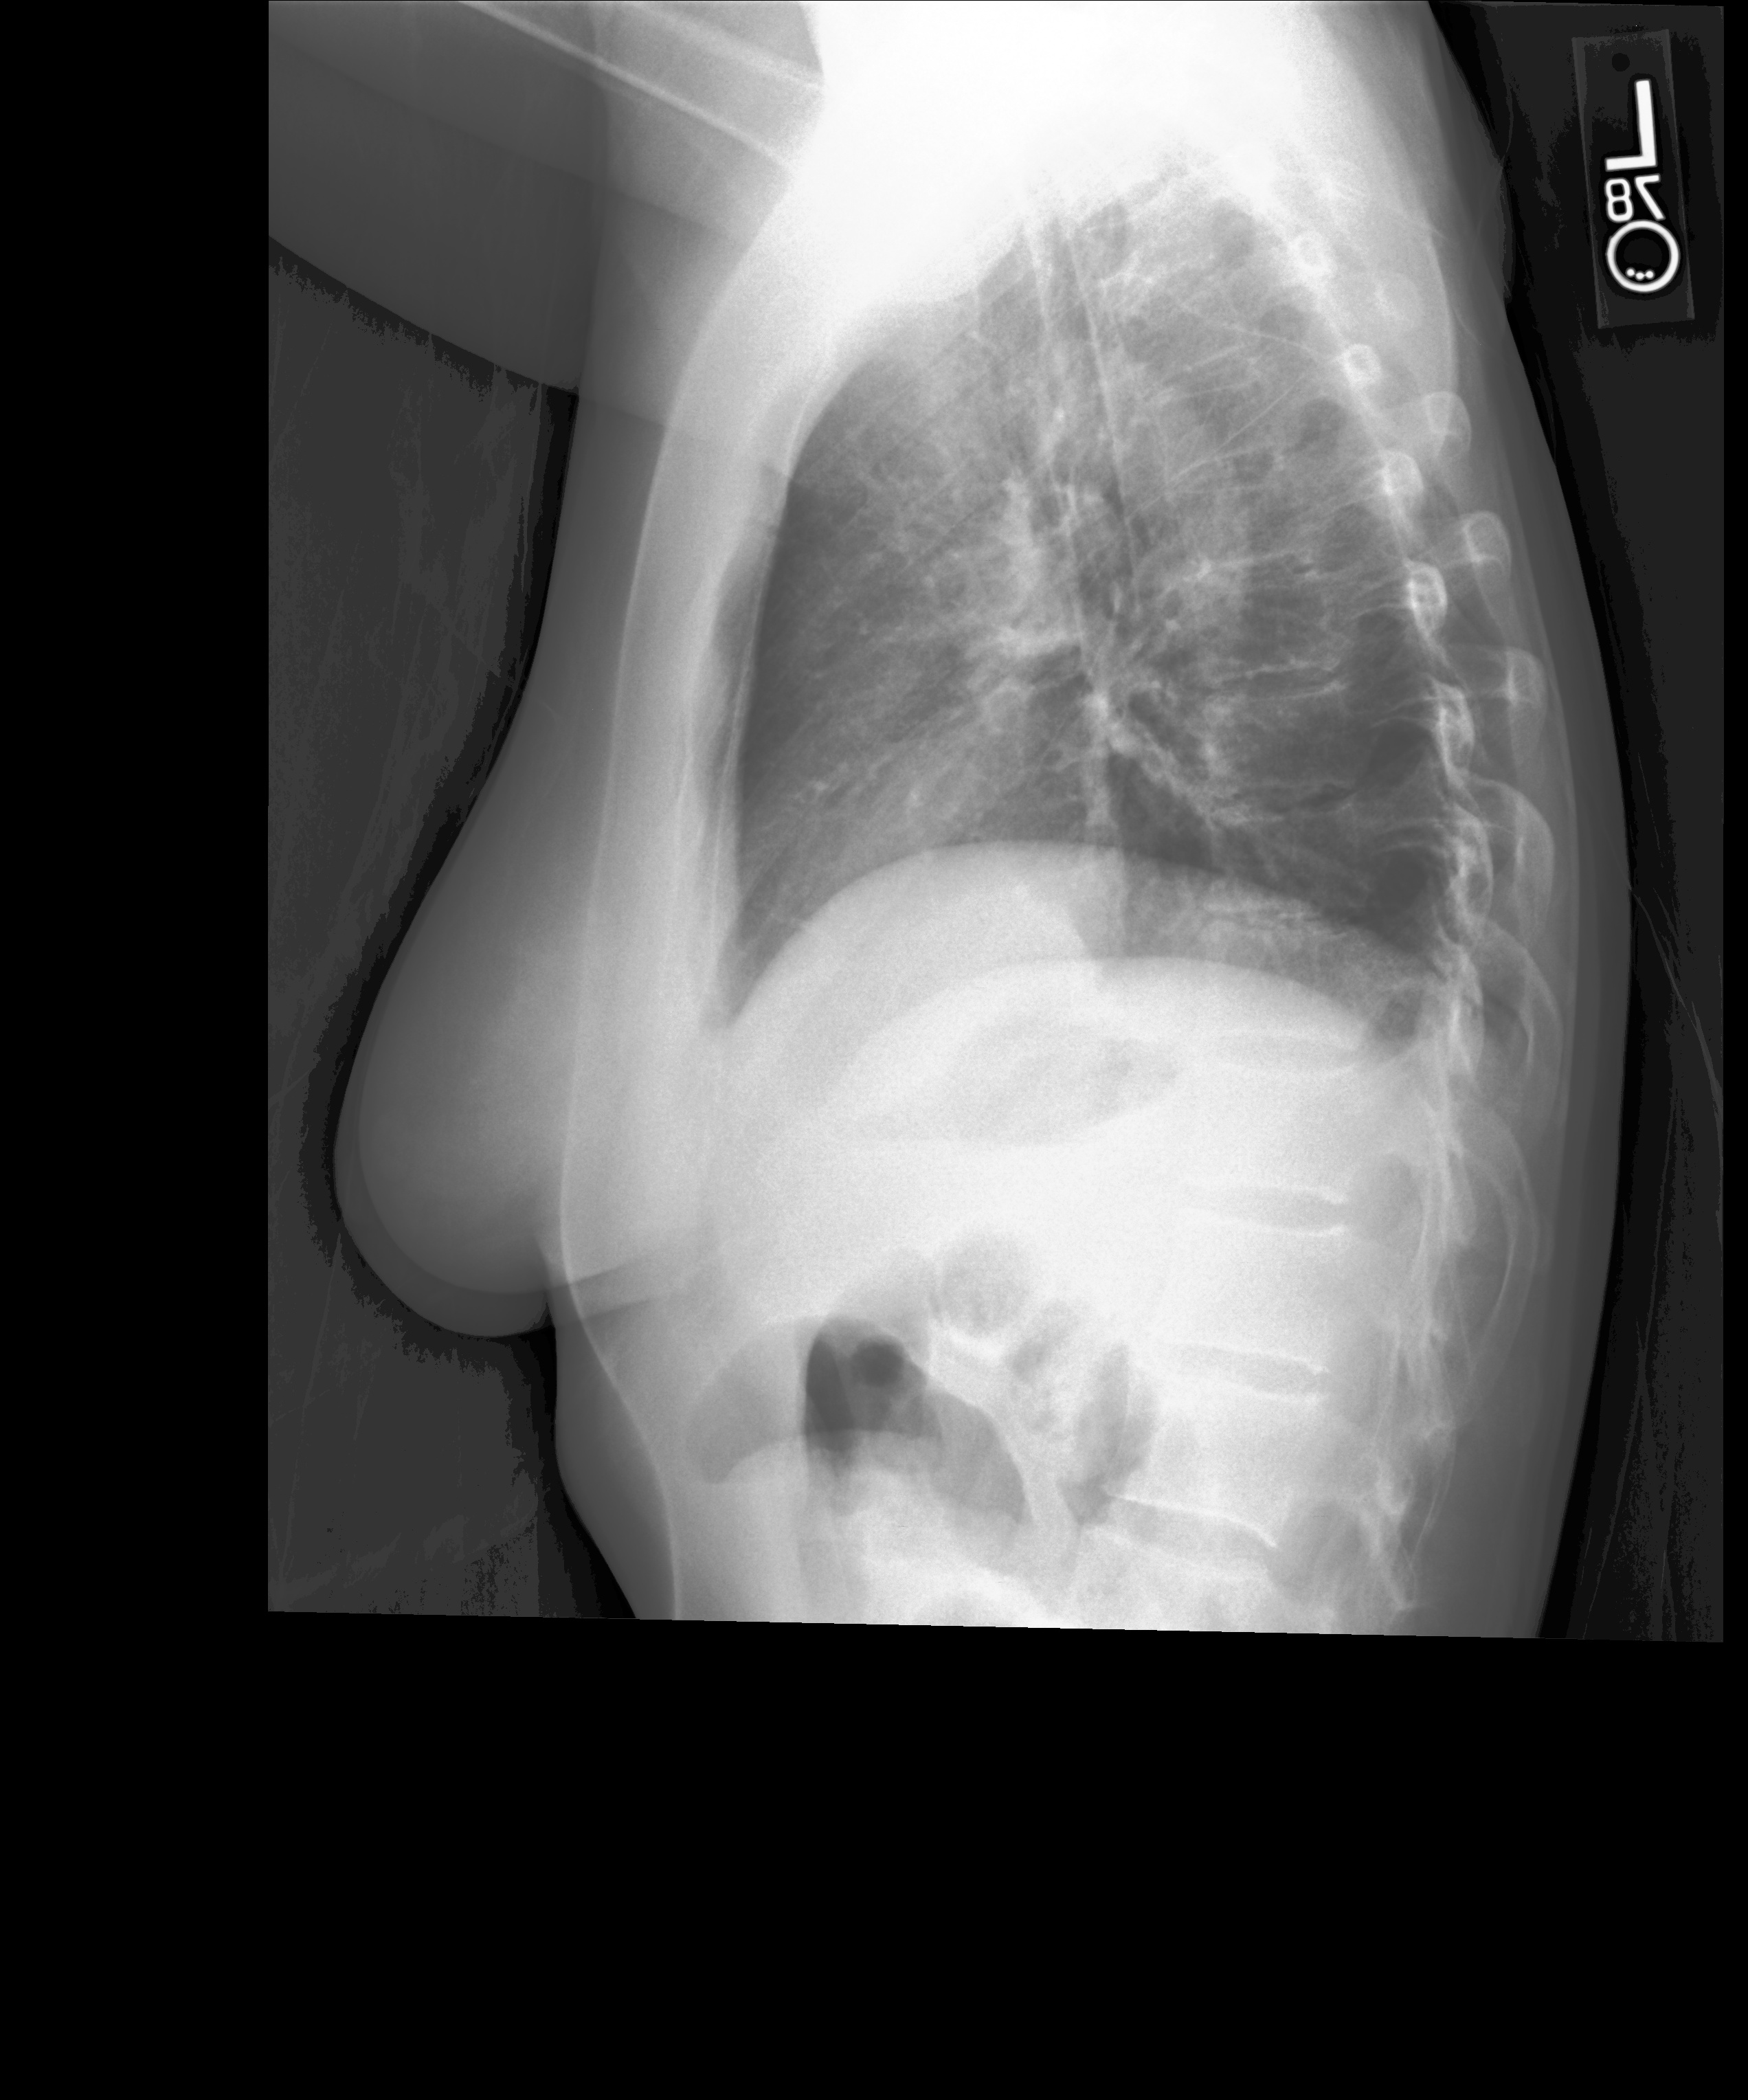
\includegraphics[width=0.45\textwidth]{images/sample_1065_2.jpg}
\end{figure}

\noindent\textbf{诊断报告对比：}

\begin{table}[h]
\small
\begin{tabular}{p{0.47\textwidth}|p{0.47\textwidth}}
\toprule
\textbf{Ground Truth} & \textbf{模型预测} \\
\midrule
Frontal and lateral views of the chest were obtained. Lungs are clear without focal consolidation. No pleural effusion or pneumothorax is seen. Cardiac and mediastinal silhouettes are unremarkable. IMPRESSION: No acute cardiopulmonary process. & IMPRESSION: In comparison with the study, there is little change and no evidence of acute cardiopulmonary disease. Mild hyperexpansion of the lungs is again seen, but no acute pneumonia, vascular congestion, or pleural effusion. \\
\midrule
\multicolumn{2}{l}{\textbf{评分：}6.0/10.0 \quad \textbf{错误类型：}遗漏（气胸）} \\
\bottomrule
\end{tabular}
\end{table}

\noindent\textbf{分析：}模型正确识别了无急性心肺疾病的主要结论。主要问题是遗漏了Ground Truth中明确指出的"无气胸"。虽然这是一个遗漏，但整体诊断方向正确，属于轻微差异。

\subsubsection{案例5：高质量预测（9.0分）}

\noindent\textbf{样本信息：}Sample ID 1115

\noindent\textbf{输入图像：}

\begin{figure}[h]
\centering
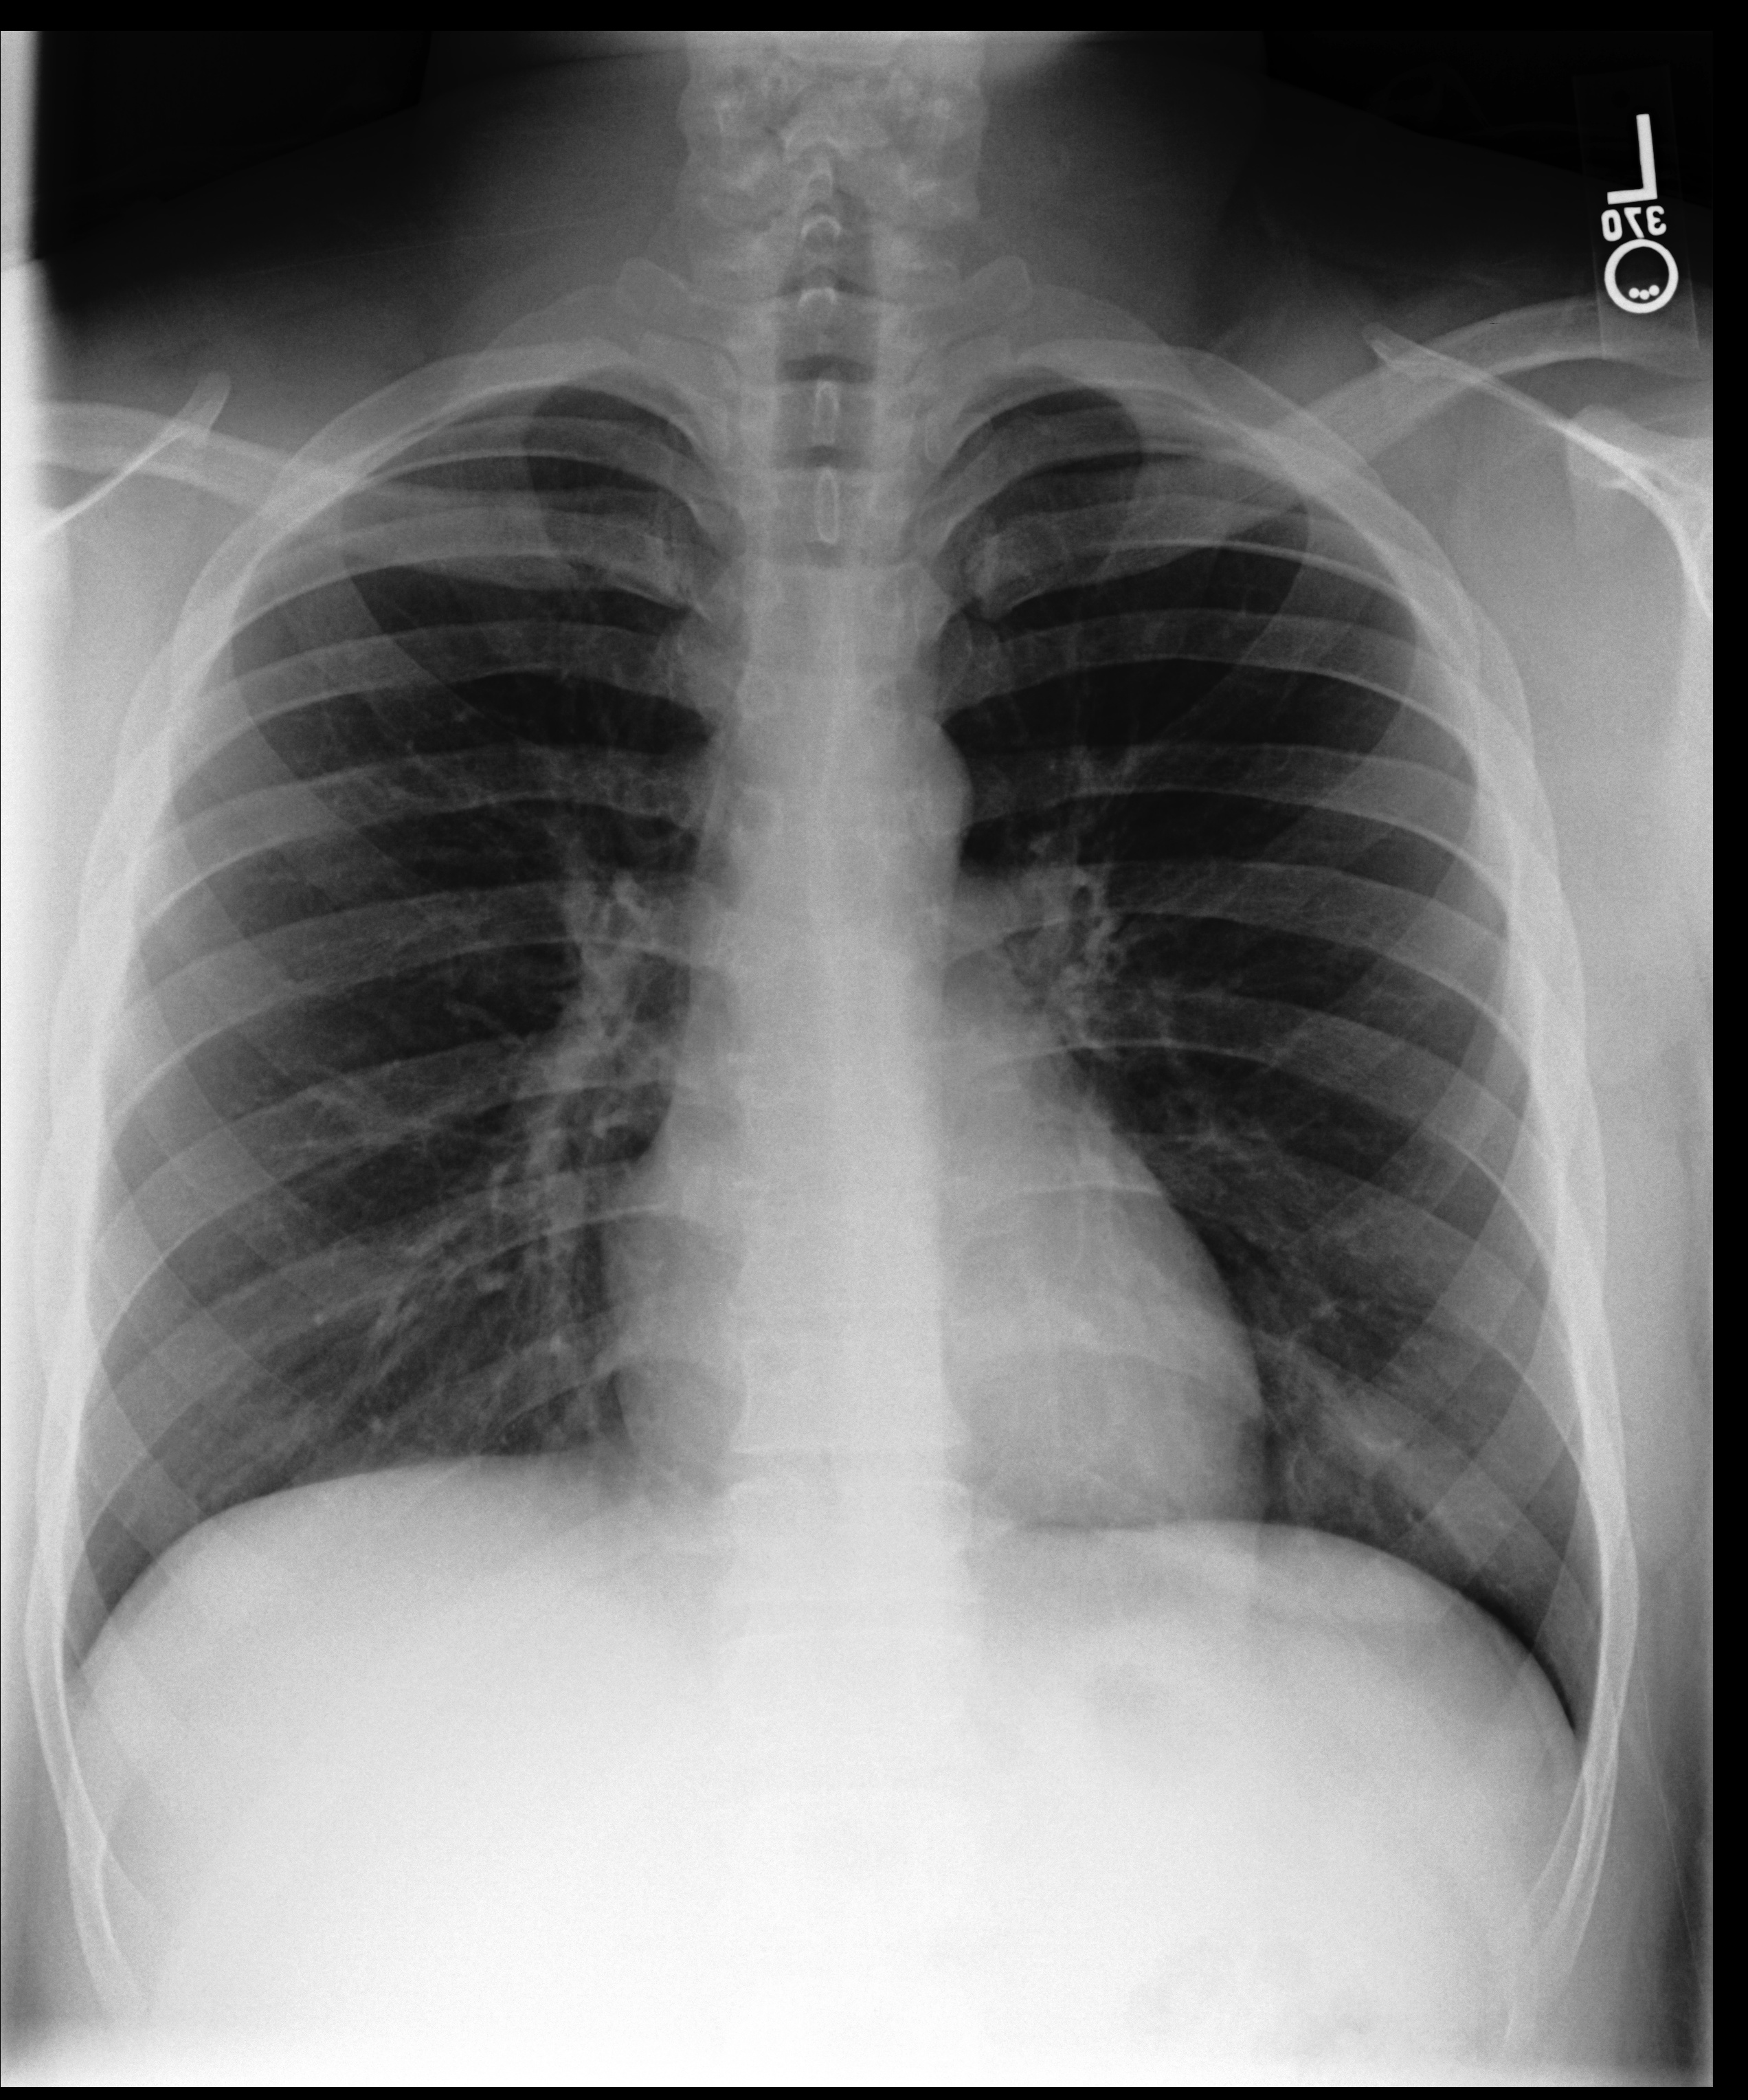
\includegraphics[width=0.45\textwidth]{images/sample_1115_1.jpg}
\hfill
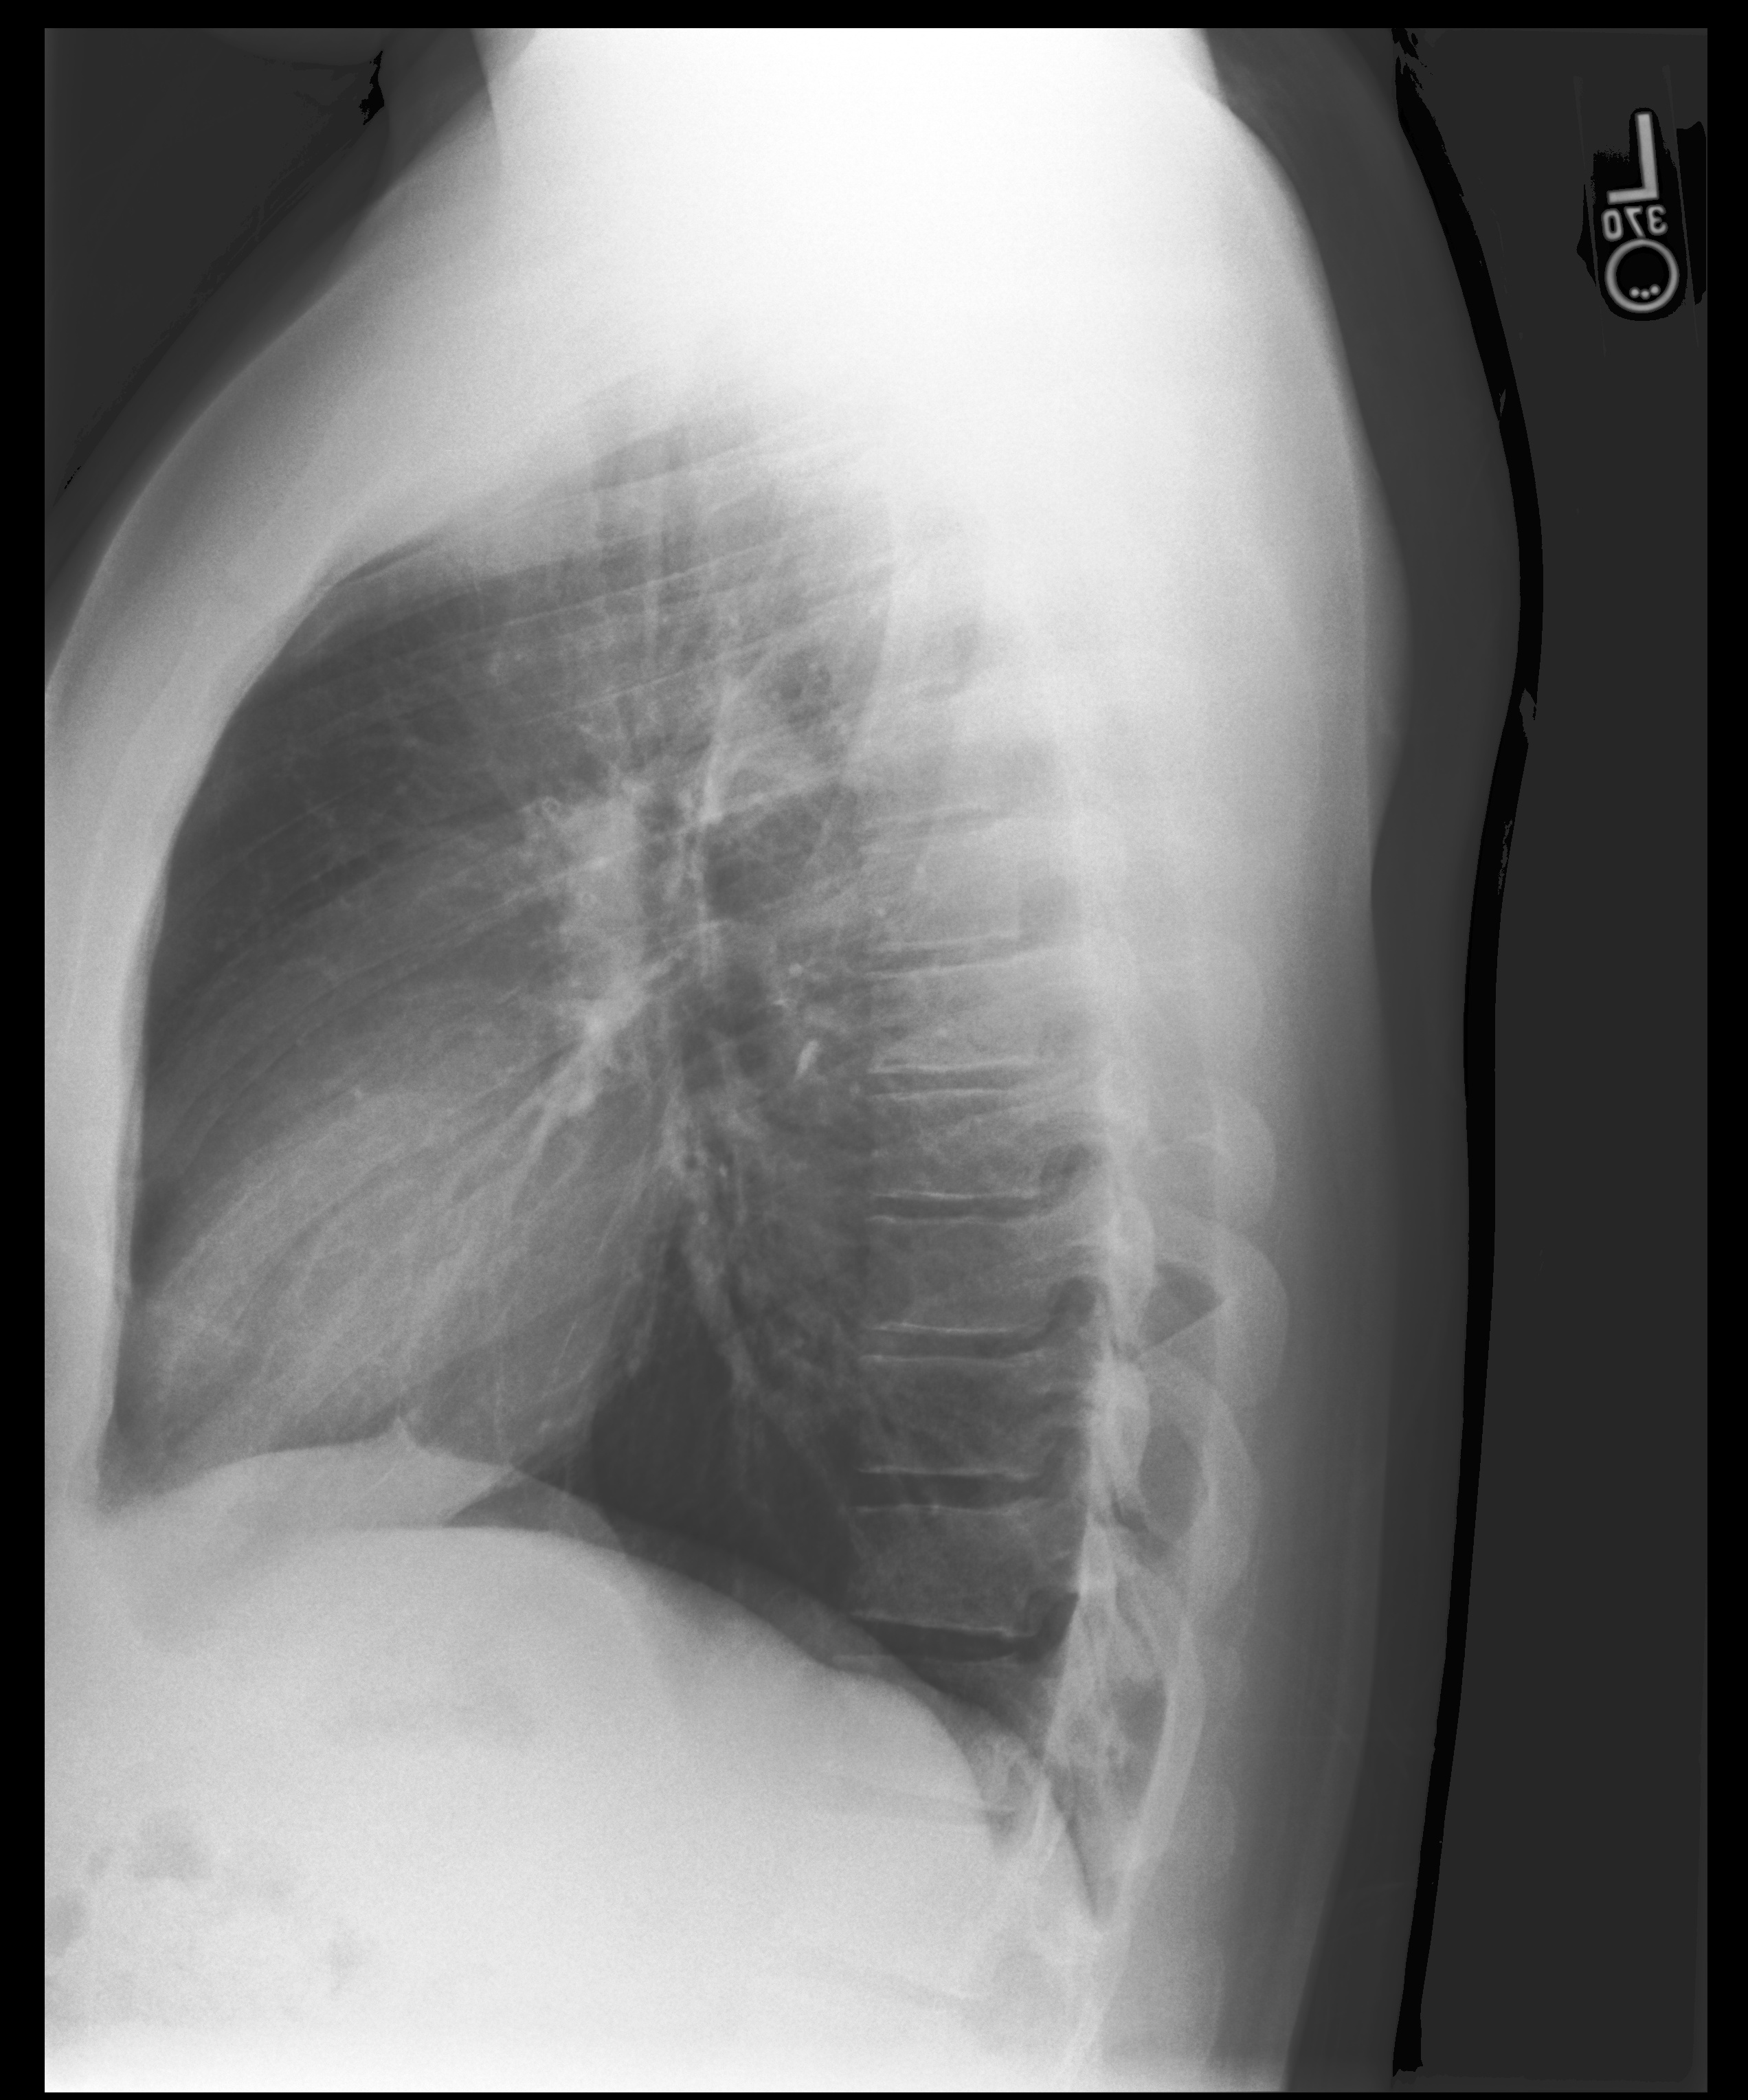
\includegraphics[width=0.45\textwidth]{images/sample_1115_2.jpg}
\end{figure}

\noindent\textbf{诊断报告对比：}

\begin{table}[h]
\small
\begin{tabular}{p{0.47\textwidth}|p{0.47\textwidth}}
\toprule
\textbf{Ground Truth} & \textbf{模型预测} \\
\midrule
Frontal and lateral views of the chest were obtained. No focal consolidation, pleural effusion, or evidence of pneumothorax is seen. The cardiac and mediastinal silhouettes are unremarkable. Hilar contours are stable. IMPRESSION: No acute cardiopulmonary process. & Frontal and lateral views of the chest were obtained. The lungs are well expanded and clear. There is no focal consolidation, pleural effusion, or pneumothorax. The cardiac and mediastinal contours are normal. The hilar structures are unremarkable. There is no free air beneath the diaphragm. IMPRESSION: No acute intrathoracic process. \\
\midrule
\multicolumn{2}{l}{\textbf{评分：}9.0/10.0 \quad \textbf{错误类型：}轻微幻觉} \\
\bottomrule
\end{tabular}
\end{table}

\noindent\textbf{分析：}模型准确识别了所有主要的阴性发现（无实变、无积液、无气胸），结论也完全正确。唯一的问题是添加了"膈下无游离气体"这一Ground Truth中未提及的描述，属于非常轻微的幻觉。整体表现接近专家水平。

\section{技术创新点}

\subsection{自动化评估流水线}

构建了从模型推理、LLM评审到推理生成的完整流水线。整个流程无需人工干预，可以自动完成大规模样本的评估工作。流水线采用模块化设计，各组件之间通过标准JSON格式进行数据交换，便于扩展和维护。

\subsection{高并发容错架构}

使用线程池实现高并发API调用，相比串行处理提速10-20倍。实现了线程安全的结果存储机制，使用锁机制防止并发写入冲突。智能重试策略采用指数退避算法（1、2、4、8、16秒），有效应对API波动。系统定期保存中间结果（每20或50个样本），防止长时间运行过程中的数据丢失。

\subsection{灵活的认证系统}

支持两种API认证方式（Basic Auth和Direct API Key），通过配置变量自动切换，适应不同的部署环境。系统根据认证模式自动选择合适的API端点和模型名称，无需手动修改代码，提高了系统的可移植性。

\subsection{结构化评审输出}

评审结果采用结构化JSON格式，包含完整的评审输入（prompt）、评审输出、错误类型分类、尝试次数等信息，便于后续的深度分析和模型改进。系统会自动处理不同模型的输出格式差异，统一提取有效的评审内容。

\section{未来工作}

短期计划包括：引入更多评估指标（BLEU、ROUGE、临床实体F1等传统NLG指标），开发评估结果可视化分析平台（交互式图表展示），实现多模型性能对比分析功能（横向对比不同规模和架构的模型），优化大规模并发处理的内存管理（减少峰值显存占用）。

长期规划包括：扩展到其他医学影像模态（CT、MRI等）以验证方法的泛化性，构建人类专家评审标注平台获取高质量的人工标注数据，开发针对性的模型安全性测试套件（对抗样本、边界情况），探索将系统集成到临床决策支持系统中实现实际应用。

\section{总结}

本阶段工作完成了从数据处理、模型训练到自动化评估的完整流程。首先使用convert\_mimic\_to\_sharegpt.py脚本将MIMIC-CXR原始数据转换为ShareGPT格式，生成19,972个训练样本和2,219个测试样本。然后基于Qwen3-VL-8B-Instruct模型进行全参数微调，采用DeepSpeed ZeRO-3优化训练，2个epoch后模型loss收敛到0.992。

在评估阶段，系统包括模型评估、LLM评审和推理生成三个核心模块，具备高并发处理能力和完善的容错机制。在2,219个MIMIC-CXR测试样本上的评估结果显示，微调后的模型在约15\%的案例上达到了8-10分的高水平，但仍有超过50\%的样本存在遗漏、幻觉等临床准确性问题。使用两个不同的LLM作为评审员，从不同角度验证了评估结果的可靠性。

该系统已具备生产级别的稳定性和性能，可支持医学影像模型的大规模自动化评估工作，为模型的安全性研究和临床应用提供重要参考。

\end{document}
